\subsection{User Design}

With health care chosen as the project's primary use case, below I consider how users would interact with a potential system and how this affects potential architecture choices. It is important to keep these choices as generic as possible for the purposes of making the project extensible for further use cases and development.

\subsubsection{User Journeys}

The below sequence diagrams show the interactions between the different entities. First I note my assumptions, followed by a specific example interaction between a patient and the health care system (the patient experiences extreme pain in their left foot) and how this might be reflected by internal transactions of information within the health care system.

Assumptions:

\begin{itemize}
  \item Interactions between the patient and doctor are assumed to be non-digital (i.e. verbal, transfer of physical data).
  \item The doctor has the ability to communicate (on behalf of a patient) with a local hospital for the purposes of referring a patient for treatment
  \item The doctor, the hospital and any existing entities represented in the health care system would have an ability to connect with modern technology likely via a connection layer between the new and in-use technology.
  \item There is a requirement that personel who act as health care professionals must validate their identity against central bodies. For doctors, this body is the GMC~\footnote{\href{http://www.gmc-uk.org/}{General Medical Council}}.
\end{itemize}

The diagrams below are split such that different entity types are represented on each side. The three entities on the left (patient, doctor, hospital) represent people interacting with the system. The three entities on the right (GMC, Patient Chain, Off-chain storage) represent technologies which act autonomously in these scenarios (according to the way they are programmed). Of note, GMC is the identity of some group on a public decentralised ledger and Patient Chain represents some instance of a blockchain of patient transactions unique to each patient.

\paragraph{Doctor requests X-ray}

The patient visits the doctor, complaining of extreme pain in their left foot. On evaluation, the doctor requests an X-ray be taken at a local hospital. Furthermore, the doctor's identification is validated before creating any transactions on the patient's chain and their signature. The data gateway hosts a local version of each patient's chain with the hospital's addresses unlocked (i.e. authenticated to make requests).

\begin{figure}[H]
  \centering
  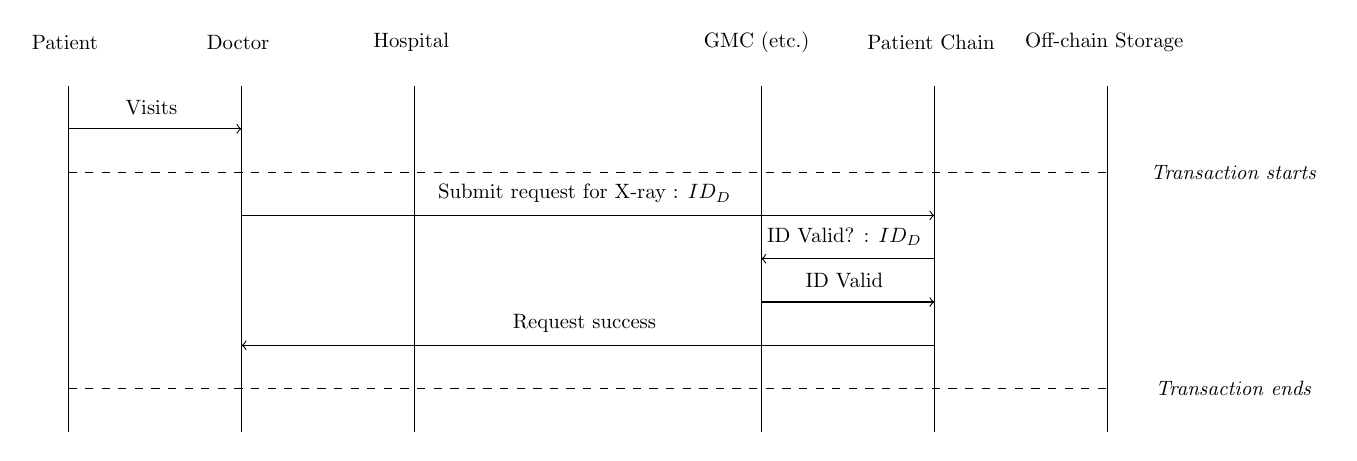
\begin{tikzpicture}[scale = 0.55, every node/.style={scale = 0.75}, every node/.append style={fill = white, rounded corners = 2pt, inner sep = 2pt, align = center}]

  % Lines
  \draw (4, 12) -- (4, 20);
  \draw (8, 12) -- (8, 20);
  \draw (12, 12) -- (12, 20);
  \draw (20, 12) -- (20, 20);
  \draw (24, 12) -- (24, 20);
  \draw (28, 12) -- (28, 20);

  % Headings
  \node at (4, 21) { Patient };
  \node at (8, 21) { Doctor };
  \node at (12, 21) { Hospital };
  \node at (20, 21) { GMC (etc.) };
  \node at (24, 21) { Patient Chain };
  \node at (28, 21) { Off-chain Storage };

  % Arrows
  \node at (6, 19.5) { Visits };
  \draw [ -> ] (4, 19) -- (8, 19);

  \node at (31, 18) { \textit{Transaction starts} };
  \draw [ dashed ] (4, 18) -- (28, 18);

  \node at (16, 17.5) { Submit request for X-ray : $ID_{D}$ };
  \draw [ -> ] (8, 17) -- (24, 17);

  \node at (22, 16.5) { ID Valid? : $ID_{D}$ };
  \draw [ -> ] (24, 16) -- (20, 16);

  \node at (22, 15.5) { ID Valid \checkmark };
  \draw [ -> ] (20, 15) -- (24, 15);

  \node at (16, 14.5) { Request success };
  \draw [ -> ] (24, 14) -- (8, 14);

  \node at (31, 13) { \textit{Transaction ends} };
  \draw [ dashed ] (4, 13) -- (28, 13);

  \end{tikzpicture}
  \caption{
    Doctor requests patient X-ray
  }{
    The doctor sends a transaction to the patient's record which creates a request file with the details of what needs to be done and the doctors notes. This will need to be accepted by the hospital.
  }
  \label{fig:user_story_01a}
\end{figure}


\begin{figure}[H]
  \centering
  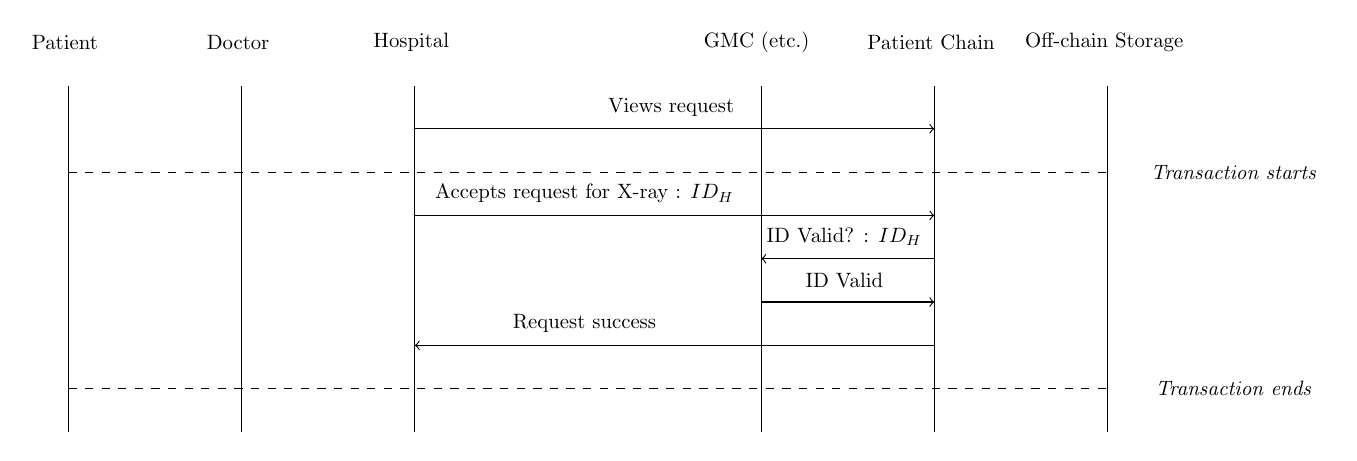
\begin{tikzpicture}[scale = 0.55, every node/.style={scale = 0.75}, every node/.append style={fill = white, rounded corners = 2pt, inner sep = 2pt, align = center}]

  % Lines
  \draw (4, 12) -- (4, 20);
  \draw (8, 12) -- (8, 20);
  \draw (12, 12) -- (12, 20);
  \draw (20, 12) -- (20, 20);
  \draw (24, 12) -- (24, 20);
  \draw (28, 12) -- (28, 20);

  % Headings
  \node at (4, 21) { Patient };
  \node at (8, 21) { Doctor };
  \node at (12, 21) { Hospital };
  \node at (20, 21) { GMC (etc.) };
  \node at (24, 21) { Patient Chain };
  \node at (28, 21) { Off-chain Storage };

  % Arrows
  \node at (18, 19.5) { Views request };
  \draw [ -> ] (12, 19) -- (24, 19);

  \node at (31, 18) { \textit{Transaction starts} };
  \draw [ dashed ] (4, 18) -- (28, 18);

  \node at (16, 17.5) { Accepts request for X-ray : $ID_{H}$ };
  \draw [ -> ] (12, 17) -- (24, 17);

  \node at (22, 16.5) { ID Valid? : $ID_{H}$ };
  \draw [ -> ] (24, 16) -- (20, 16);

  \node at (22, 15.5) { ID Valid \checkmark };
  \draw [ -> ] (20, 15) -- (24, 15);

  \node at (16, 14.5) { Request success };
  \draw [ -> ] (24, 14) -- (12, 14);

  \node at (31, 13) { \textit{Transaction ends} };
  \draw [ dashed ] (4, 13) -- (28, 13);

  \end{tikzpicture}
  \caption{
    Hospital accepts a doctor's request for an X-ray
  }{
    The hospital accepts the request, made by the doctor, for the patient's X-ray. This paves the way for the hospital and the patient to negotiate a time for the appointment. \textit{Note: whilst the hospital is shown as having some $ID_{H}$ above, in reality this might be the id of an administrator of X-ray requests who is a member of a hospital administration group (similar to the GMC for doctors).}
  }
  \label{fig:user_story_01b}
\end{figure}


\paragraph{Patient has X-ray taken}

The next step in the process is for the X-ray to be taken. The patient visits the hospital where the doctor has referred them and has the X-ray taken, with the data being securely stored in off-chain storage and logged in the patient's chain. Note that this portion of the user journey requires the most transactions to be committed and mined.

\begin{figure}[H]
  \centering
  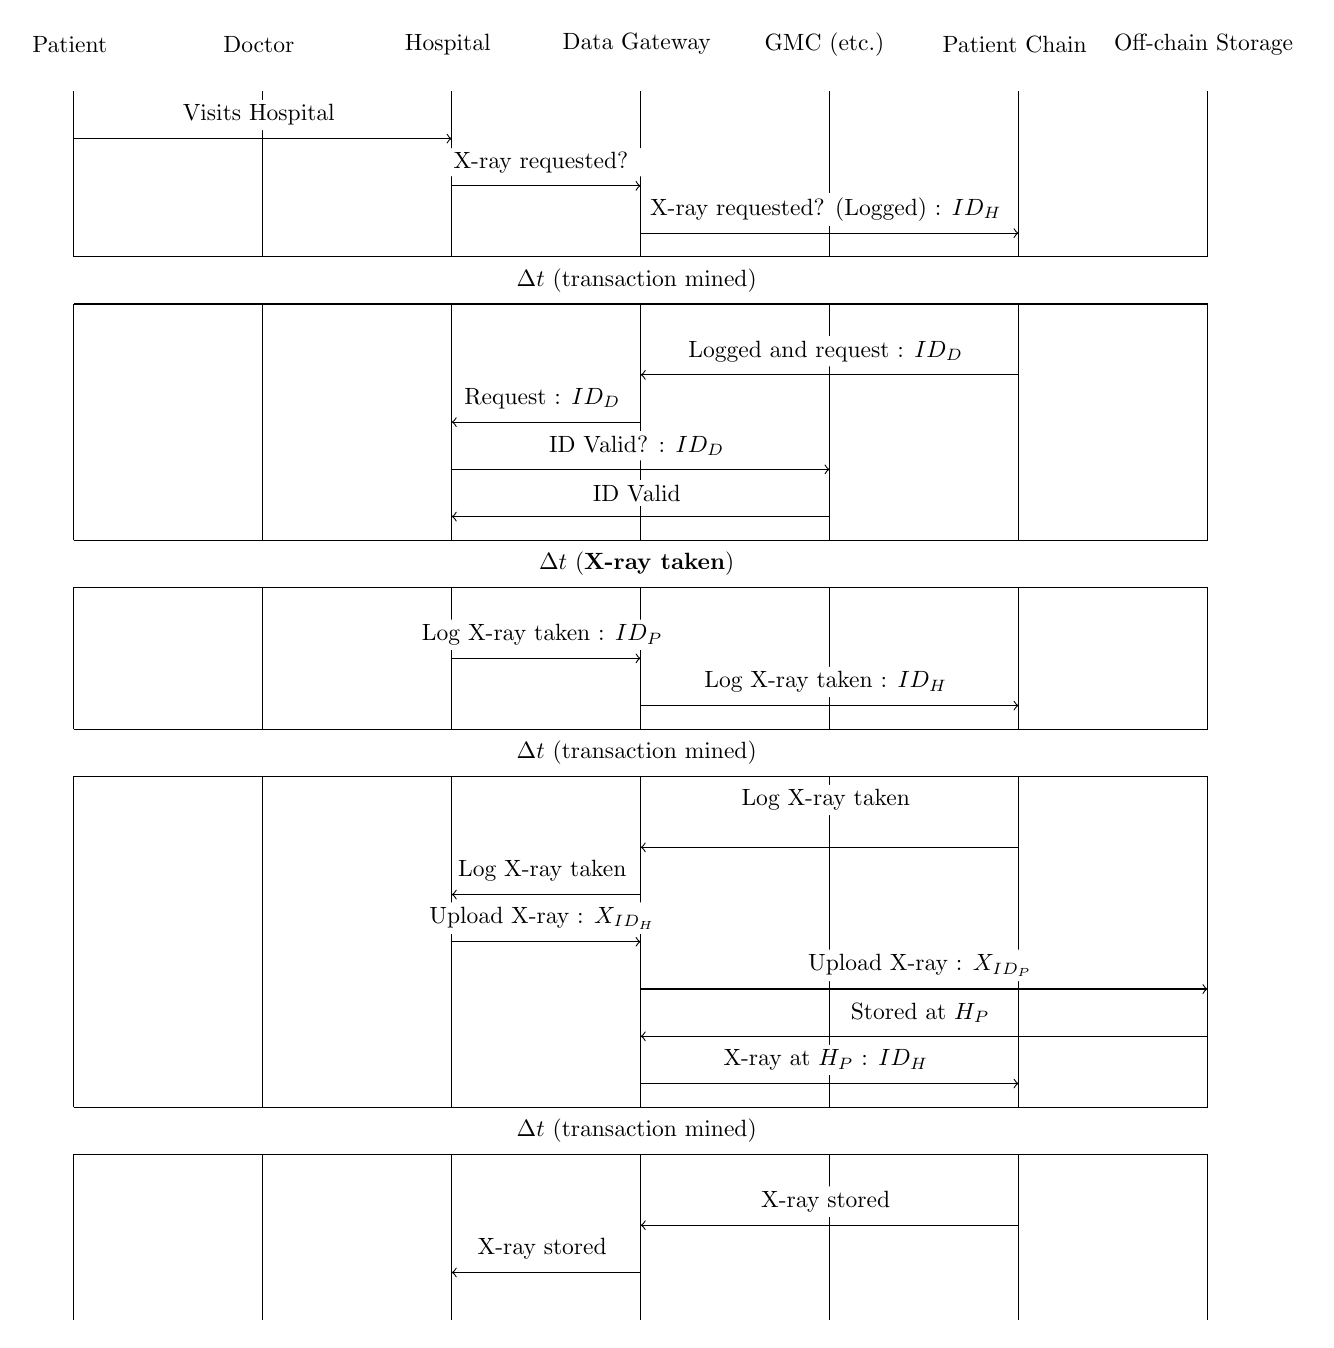
\begin{tikzpicture}[scale = 0.6, every node/.style={scale = 0.85}, every node/.append style={fill = white, rounded corners = 2pt, inner sep = 2pt, align = center}]

  % Lines
  \draw (4, -6) -- (4, -2.5);
  \draw (4, -1.5) -- (4, 5.5);
  \draw (4, 6.5) -- (4, 9.5);
  \draw (4, 10.5) -- (4, 15.5);
  \draw (4, 16.5) -- (4, 20);
  \draw (8, -6) -- (8, -2.5);
  \draw (8, -1.5) -- (8, 5.5);
  \draw (8, 6.5) -- (8, 9.5);
  \draw (8, 10.5) -- (8, 15.5);
  \draw (8, 16.5) -- (8, 20);
  \draw (12, -6) -- (12, -2.5);
  \draw (12, -1.5) -- (12, 5.5);
  \draw (12, 6.5) -- (12, 9.5);
  \draw (12, 10.5) -- (12, 15.5);
  \draw (12, 16.5) -- (12, 20);
  \draw (16, -6) -- (16, -2.5);
  \draw (16, -1.5) -- (16, 5.5);
  \draw (16, 6.5) -- (16, 9.5);
  \draw (16, 10.5) -- (16, 15.5);
  \draw (16, 16.5) -- (16, 20);
  \draw (20, -6) -- (20, -2.5);
  \draw (20, -1.5) -- (20, 5.5);
  \draw (20, 6.5) -- (20, 9.5);
  \draw (20, 10.5) -- (20, 15.5);
  \draw (20, 16.5) -- (20, 20);
  \draw (24, -6) -- (24, -2.5);
  \draw (24, -1.5) -- (24, 5.5);
  \draw (24, 6.5) -- (24, 9.5);
  \draw (24, 10.5) -- (24, 15.5);
  \draw (24, 16.5) -- (24, 20);
  \draw (28, -6) -- (28, -2.5);
  \draw (28, -1.5) -- (28, 5.5);
  \draw (28, 6.5) -- (28, 9.5);
  \draw (28, 10.5) -- (28, 15.5);
  \draw (28, 16.5) -- (28, 20);

  % Headings
  \node at (4, 21) { Patient };
  \node at (8, 21) { Doctor };
  \node at (12, 21) { Hospital };
  \node at (16, 21) { Data Gateway };
  \node at (20, 21) { GMC (etc.) };
  \node at (24, 21) { Patient Chain };
  \node at (28, 21) { Off-chain Storage };

  % Arrows
  \node at (8, 19.5) { Visits Hospital };
  \draw [ -> ] (4, 19) -- (12, 19);

  \node at (14, 18.5) { X-ray requested? };
  \draw [ -> ] (12, 18) -- (16, 18);

  \node at (20, 17.5) { X-ray requested? (Logged) : $ID_{H}$ };
  \draw [ -> ] (16, 17) -- (24, 17);

  \draw (4, 16.5) -- (28, 16.5);
  \node at (16, 16) { $\Delta t$ (transaction mined) };
  \draw (4, 15.5) -- (28, 15.5);

  \node at (20, 14.5) { Logged \checkmark and request : $ID_{D}$ };
  \draw [ -> ] (24, 14) -- (16, 14);

  \node at (14, 13.5) { Request : $ID_{D}$ };
  \draw [ -> ] (16, 13) -- (12, 13);

  \node at (16, 12.5) { ID Valid? : $ID_{D}$ };
  \draw [ -> ] (12, 12) -- (20, 12);

  \node at (16, 11.5) { ID Valid \checkmark };
  \draw [ -> ] (20, 11) -- (12, 11);

  \draw (4, 10.5) -- (28, 10.5);
  \node at (16, 10) { $\Delta t$ (\textbf{X-ray taken}) };
  \draw (4, 9.5) -- (28, 9.5);

  \node at (14, 8.5) { Log X-ray taken : $ID_{P}$ };
  \draw [ -> ] (12, 8) -- (16, 8);

  \node at (20, 7.5) { Log X-ray taken : $ID_{H}$ };
  \draw [ -> ] (16, 7) -- (24, 7);

  \draw (4, 6.5) -- (28, 6.5);
  \node at (16, 6) { $\Delta t$ (transaction mined) };
  \draw (4, 5.5) -- (28, 5.5);

  \node at (20, 5) { Log X-ray taken \checkmark };
  \draw [ -> ] (24, 4) -- (16, 4);

  \node at (14, 3.5) { Log X-ray taken \checkmark };
  \draw [ -> ] (16, 3) -- (12, 3);

  \node at (14, 2.5) { Upload X-ray : $X_{ID_{H}}$ };
  \draw [ -> ] (12, 2) -- (16, 2);

  \node at (22, 1.5) { Upload X-ray : $X_{ID_{P}}$ };
  \draw [ -> ] (16, 1) -- (28, 1);

  \node at (22, 0.5) { Stored at $H_{P}$ };
  \draw [ -> ] (28, 0) -- (16, 0);

  \node at (20, -0.5) { X-ray at $H_{P}$ : $ID_{H}$ };
  \draw [ -> ] (16, -1) -- (24, -1);

  \draw (4, -1.5) -- (28, -1.5);
  \node at (16, -2) { $\Delta t$ (transaction mined) };
  \draw (4, -2.5) -- (28, -2.5);

  \node at (20, -3.5) { X-ray stored \checkmark };
  \draw [ -> ] (24, -4) -- (16, -4);

  \node at (14, -4.5) { X-ray stored \checkmark };
  \draw [ -> ] (16, -5) -- (12, -5);

  \end{tikzpicture}
  \caption{
    Patient visits hospital to have X-ray taken
  }
  \label{fig:user_story_02}
\end{figure}


\paragraph{Doctor views (and discusses) X-ray}

With the X-ray having been taken, processed, and likely somewhat analysed, the doctor now needs to discuss the X-ray with the patient to communicate any further treatment required etc. Through this part of the process the doctor's access is logged before the data is retrieved.

\begin{figure}[H]
  \centering
  \begin{tikzpicture}[scale = 0.6, every node/.style={scale = 0.85}, every node/.append style={fill = white, rounded corners = 2pt, inner sep = 2pt, align = center}]

  % Lines
  \draw (4, 2) -- (4, 20);
  \draw (8, 2) -- (8, 20);
  \draw (12, 2) -- (12, 20);
  \draw (20, 2) -- (20, 20);
  \draw (24, 2) -- (24, 20);
  \draw (28, 2) -- (28, 20);

  % Headings
  \node at (4, 21) { Patient };
  \node at (8, 21) { Doctor };
  \node at (12, 21) { Hospital };
  \node at (20, 21) { GMC (etc.) };
  \node at (24, 21) { Patient Chain };
  \node at (28, 21) { Off-chain Storage };

  % Arrows
  \node at (6, 19.5) { Visits };
  \draw [ -> ] (4, 19) -- (8, 19);

  \node at (16, 18.5) { Get X-ray address : $ID_{D}$ };
  \draw [ -> ] (8, 18) -- (24, 18);

  \node at (22, 17.5) { ID Valid? : $ID_{D}$ };
  \draw [ -> ] (24, 17) -- (20, 17);

  \node at (22, 16.5) { ID Valid \checkmark };
  \draw [ -> ] (20, 16) -- (24, 16);

  \node at (16, 15.5) { X-ray address : $H_{\text{X-ray}}$ };
  \draw [ -> ] (24, 15) -- (8, 15);

  \node at (18, 14.5) { Get X-ray Data : $H_{\text{X-ray}}$ };
  \draw [ -> ] (8, 14) -- (28, 14);

  \node at (20, 14.5) { X-ray stored \checkmark : $H_{\text{X-ray}}$ };
  \draw [ -> ] (28, 14) -- (12, 14);

  \node at (31, 13) { \textit{Transaction starts} };
  \draw [ dashed ] (4, 13) -- (28, 13);

  \node at (18, 12.5) { Add X-ray Data : $H_{\text{X-ray}}$, $ID_{H}$ };
  \draw [ -> ] (12, 12) -- (24, 12);

  \node at (22, 11.5) { ID Valid? : $ID_{H}$ };
  \draw [ -> ] (24, 11) -- (20, 11);

  \node at (22, 10.5) { ID Valid \checkmark };
  \draw [ -> ] (20, 10) -- (24, 10);

  \node at (18, 9.5) { Request success };
  \draw [ -> ] (24, 9) -- (12, 9);

  \node at (31, 8) { \textit{Transaction ends} };
  \draw [ dashed ] (4, 8) -- (28, 8);

  \end{tikzpicture}
  \caption{Doctor views X-ray with patient}{
  	The patient visits the doctor to discuss their X-ray results. The doctor gets the latest version (address / hash) of their X-ray data from their record and using this gets the X-ray data itself from off-chain storage. The doctor is then able to discuss the results with the patient (and make further edits - \textit{not shown}.
  }
  \label{fig:user_story_03}
\end{figure}


\paragraph{Patient views their log}

\begin{figure}[H]
  \centering
  \begin{tikzpicture}[scale = 0.6, every node/.style={scale = 0.85}]

  % Lines
  \draw (4, 4) -- (4, 20);
  \draw (8, 4) -- (8, 20);
  \draw (12, 4) -- (12, 20);
  \draw (16, 4) -- (16, 20);
  \draw (20, 4) -- (20, 20);
  \draw (24, 4) -- (24, 20);
  \draw (28, 4) -- (28, 20);

  % Headings
  \node[fill = white, rounded corners = 2pt, inner sep = 2pt, align = center] at (4, 21) { Patient };
  \node[fill = white, rounded corners = 2pt, inner sep = 2pt, align = center] at (8, 21) { Doctor };
  \node[fill = white, rounded corners = 2pt, inner sep = 2pt, align = center] at (12, 21) { Hospital };
  \node[fill = white, rounded corners = 2pt, inner sep = 2pt, align = center] at (16, 21) { Data Gateway };
  \node[fill = white, rounded corners = 2pt, inner sep = 2pt, align = center] at (20, 21) { GMC (etc.) };
  \node[fill = white, rounded corners = 2pt, inner sep = 2pt, align = center] at (24, 21) { Patient Chain };
  \node[fill = white, rounded corners = 2pt, inner sep = 2pt, align = center] at (28, 21) { Off-chain Storage };

  \end{tikzpicture}
  \caption{
    Doctor requests that patient have X-ray taken
  }
  \label{fig:user_story_04}
\end{figure}


\begin{figure}[H]
  \centering
  \begin{tikzpicture}[scale = 0.6, every node/.style={scale = 0.85}]

  % Lines
  \draw (4, 4) -- (4, 20);
  \draw (8, 4) -- (8, 20);
  \draw (12, 4) -- (12, 20);
  \draw (16, 4) -- (16, 20);
  \draw (20, 4) -- (20, 20);
  \draw (24, 4) -- (24, 20);
  \draw (28, 4) -- (28, 20);

  % Headings
  \node[fill = white, rounded corners = 2pt, inner sep = 2pt, align = center] at (4, 21) { Patient };
  \node[fill = white, rounded corners = 2pt, inner sep = 2pt, align = center] at (8, 21) { Doctor };
  \node[fill = white, rounded corners = 2pt, inner sep = 2pt, align = center] at (12, 21) { Hospital };
  \node[fill = white, rounded corners = 2pt, inner sep = 2pt, align = center] at (16, 21) { Data Gateway };
  \node[fill = white, rounded corners = 2pt, inner sep = 2pt, align = center] at (20, 21) { GMC (etc.) };
  \node[fill = white, rounded corners = 2pt, inner sep = 2pt, align = center] at (24, 21) { Patient Chain };
  \node[fill = white, rounded corners = 2pt, inner sep = 2pt, align = center] at (28, 21) { Off-chain Storage };

  \end{tikzpicture}
  \caption{
    Doctor requests that patient have X-ray taken
  }
  \label{fig:user_story_04}
\end{figure}

